\begin{enumerate}
	\item 
	نشان دهید هر دو مدار نشان‌داده‌شده در این سؤال یک تابع را نمایش می‌دهند. 
	
	\begin{figure}[h]
		\centering
		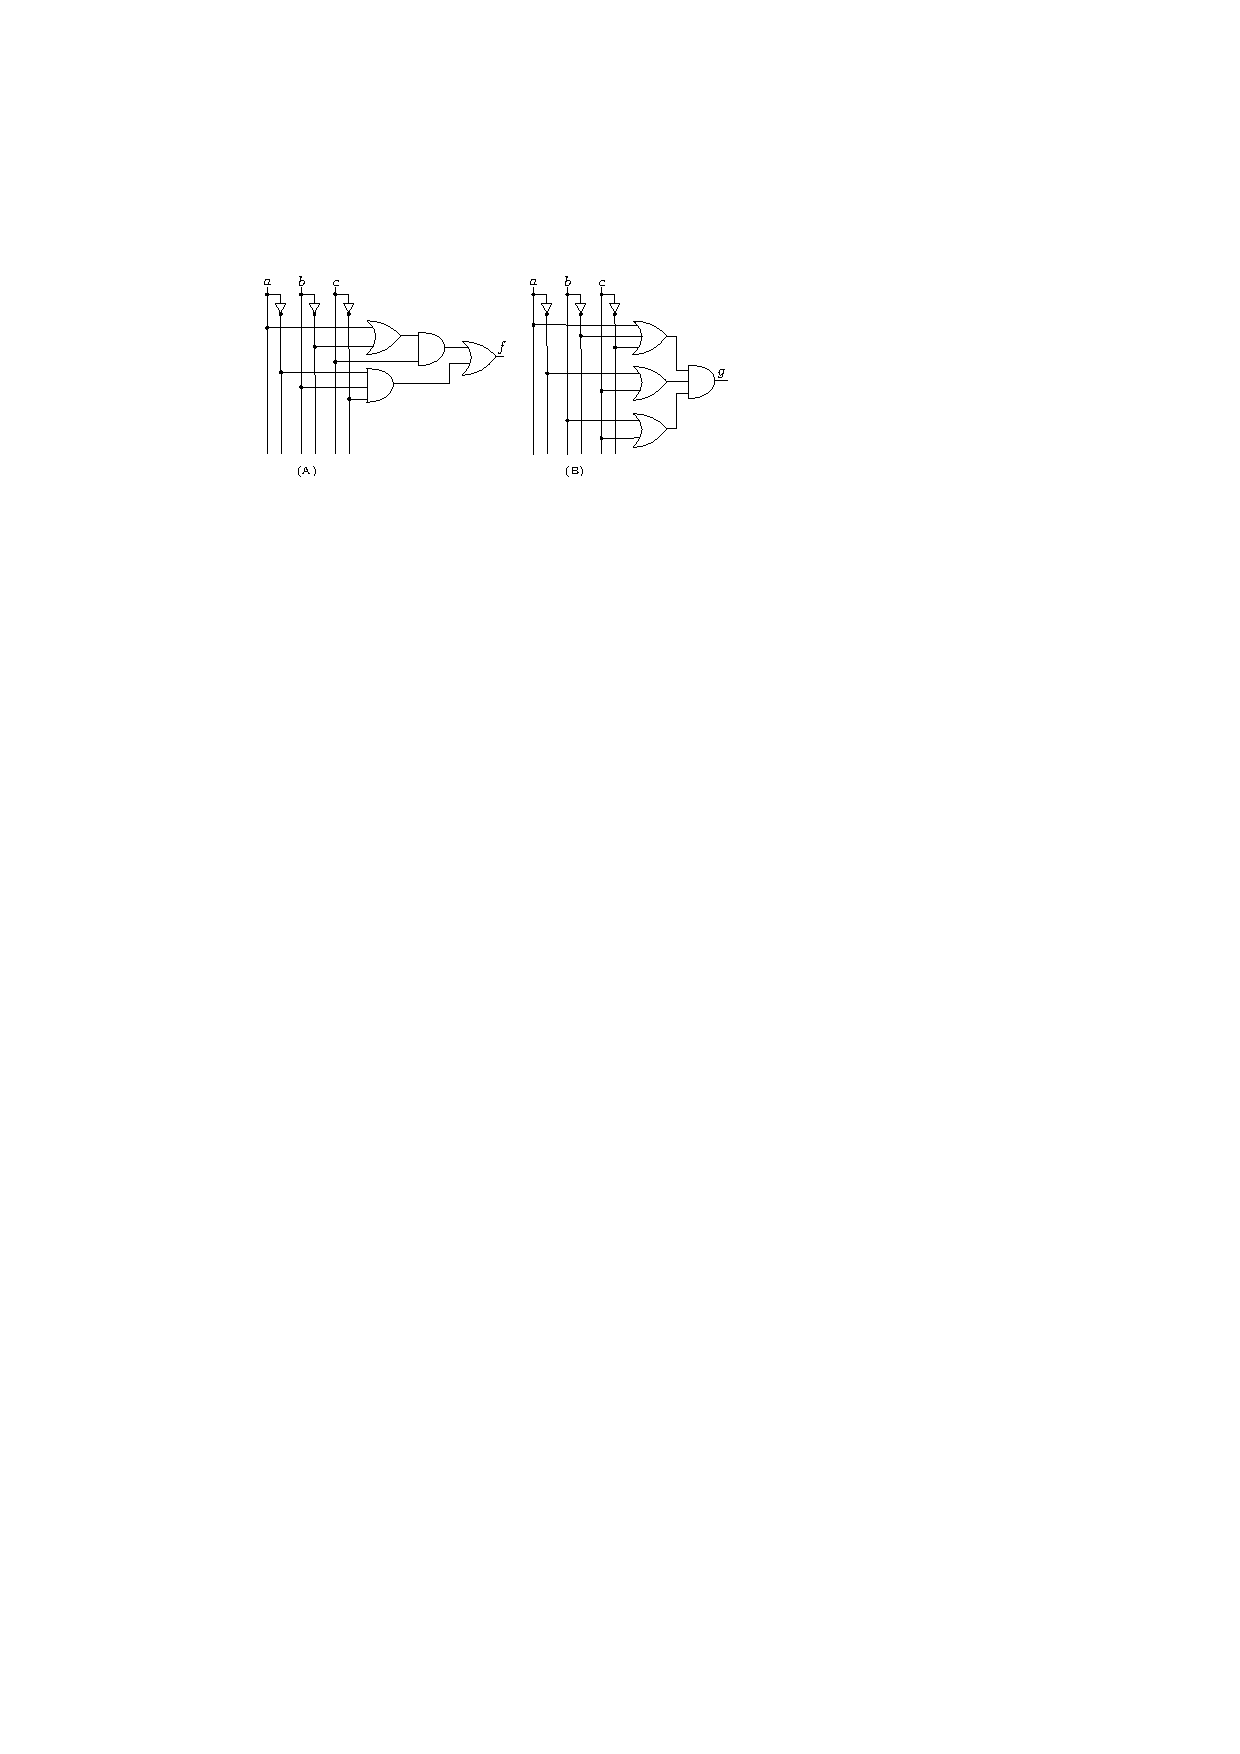
\includegraphics[width=0.9\textwidth]{fig/Q3_b.pdf}
		\label{fig:Q6_a}
	\end{figure}
	
	\item 
	شکل موج خروجی $f$ را به‌ازای سیگنال‌های ورودی داده شده رسم کنید.
	
	\begin{figure}[h]
		\centering
		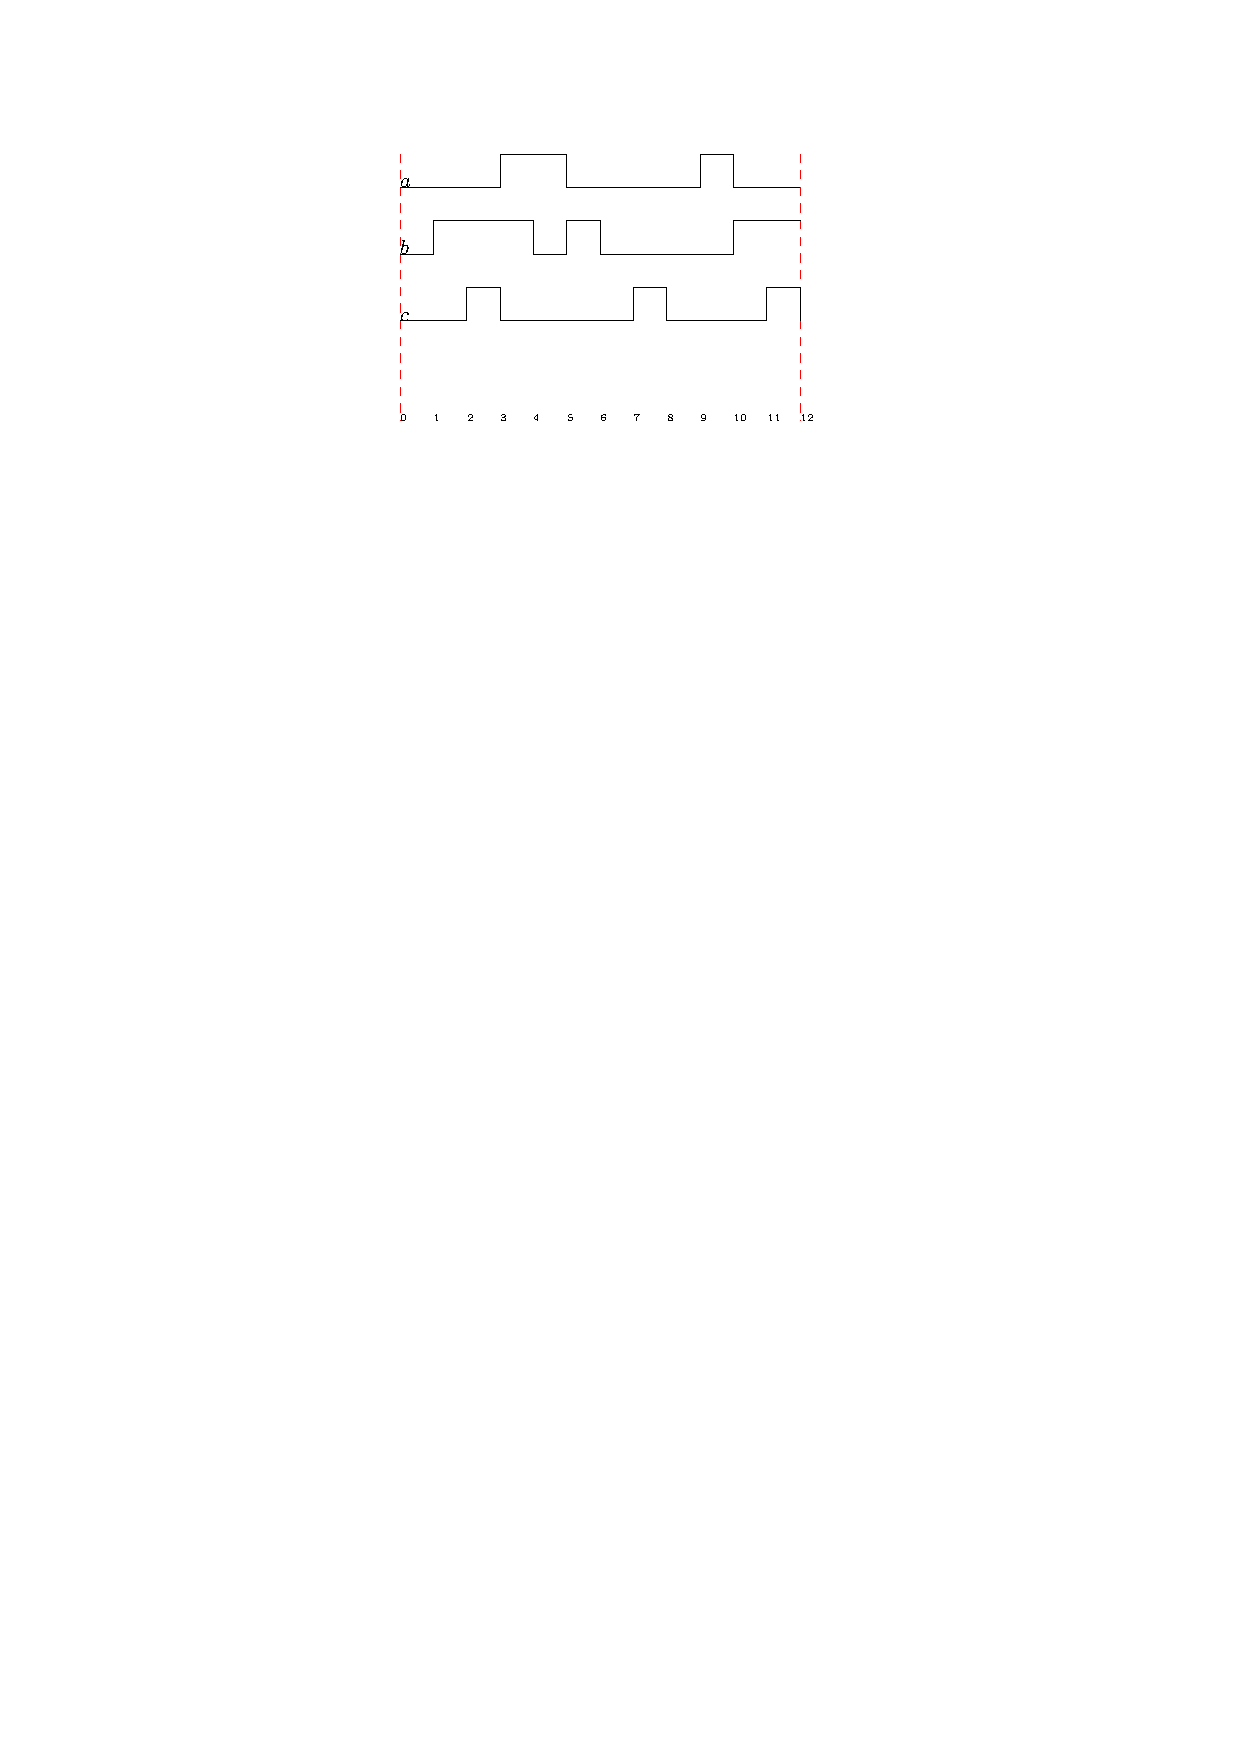
\includegraphics[width=0.9\textwidth]{fig/Q6.pdf}
		\label{fig:Q6_b}
	\end{figure}
	
\end{enumerate}